%\vspace{1cm}
\section*{Introducción}
La guía pasada estudiamos los oepradores de Sturm-Liouville y algunos problemas importantes relacionados con ellos. En esta guía, se estudiará uno de los problemas más importantes relacionados con operadores de Sturm-Liouville, la ecuación de Legendre.


\section*{Polinomios de Legendre}
Existen varias formas de inciar el estudio de los polinomios de Legendre, una de ellas es resolver la conocida ecuación de Legendre
	\begin{equation}
		\dv{x} \qty[(1 - x^2) \dv{y}{x}] + n(n + 1)y = 0, \label{eqlegendre}
	\end{equation}
y planteando una solución en forma de serie de potencia (como se muestra en el libro \textit{Mathematical Methods for Physicists: A concise introduction}, Chow, p296)
	$$ y = \sum _{m = 0} ^\infty a_m x^m. $$
Sin embargo, nosotros inicaremos a partir del problema del potencial.

\begin{figure}[H]
	\centering
	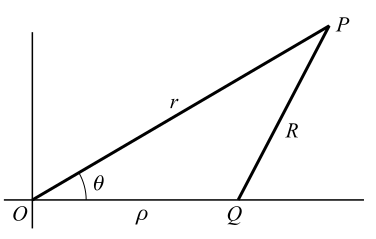
\includegraphics[scale=0.5]{./img/potential.png}
	\caption{Figura 7.2. \textit{Mathematical Methods for Physicists: A concise introduction}, Chow, p302}
	\label{potential}
\end{figure}

El potencial $V$ de una carga puntual en el punto $P$ dada una carga $+q$ en un punto $Q$, está dado por la ecuación
	$$ V_p = \frac{q}{R} = \frac{q}{(\rho ^2 - 2r\rho \cos{\theta} + r^2)^{-1/2}}, $$
entonces, se tiene (por simplicidad tomaremos una carga unitaria)
	$$
		\left.\begin{array}{ccc}
			V = \dfrac{1}{\rho} \dfrac{1}{\sqrt{1 - 2\xi \cos{\theta} + \xi ^2}}, & \xi = \dfrac{r}{\rho}, & r < \rho \\
			 & & \\
			V = \dfrac{1}{r} \dfrac{1}{\sqrt{1 - 2\xi\cos{\theta} + \xi ^2}}, & \xi = \dfrac{\rho}{r}, & r > \rho .
		\end{array}\right.
	$$



\begin{mdframed}[style=warning]
	{\Large \textbf{Función Generatriz de los Polinomios de Legendre:}} \\
		$$ \psi (x,\xi) = \frac{1}{\sqrt{1 - 2x\xi + \xi ^2}}, $$
	se le llama función generatriz dado que los polinomios de Legendre se definen como los coeficientes del desarrollo en series de potencias de $\xi$:
		\begin{equation}
			\psi (x,\xi) = \frac{1}{\sqrt{1 - 2x\xi + \xi ^2}} = \sum _{n = 0} ^\infty P_n (x) \xi ^n . \label{generatriz}
		\end{equation}
\end{mdframed}


Con esto, se tiene que
	$$
		\left.\begin{array}{cc}
			\dfrac{1}{R} = \dfrac{1}{\rho} \sum _{n = 0} ^\infty P_n (\cos{\theta}) \qty(\dfrac{r}{\rho})^n , & r < \rho \\
			 & \\
			\dfrac{1}{R} = \dfrac{1}{r} \sum _{n = 0} ^\infty P_n (\cos{\theta}) \qty(\dfrac{\rho}{r})^n, & r > \rho .
		\end{array}\right.
	$$
a lo que más se conocerá como \textbf{Armónicos Esféricos}, los cuales son la solución fundamental a la ecuación de Laplace.



\begin{mdframed}[style=warning]
	{\Large \textbf{Fórmula de Rodrigues:}} \\
	La fórma polinomial de los porlinomios de Legendre es conocida como la Fórmula de Rodrigues\footnote{Vease el desarrollo hecho en la sección 3.1.2. del libro \textit{Métodos Matemáticos de la Física.}, Marín Antuña.}.
		$$ P_n (x) = \frac{1}{2^n n!} \dv[n]{x} \qty[(x^2 - 1)^n]. $$
	Existe otra forma de expresar los polinomios de Legendre, es poco útil, pero no está de más mencionarla
		$$ P_n (x) = \sum _{k = 0} ^{\lceil n/2 \rceil} (-1)^k \frac{(2n - 2k)!}{2^n k! (n - k)! (n - 2k)!} x^{n - 2k}. $$
\end{mdframed}




\begin{figure}[H]
	\centering
	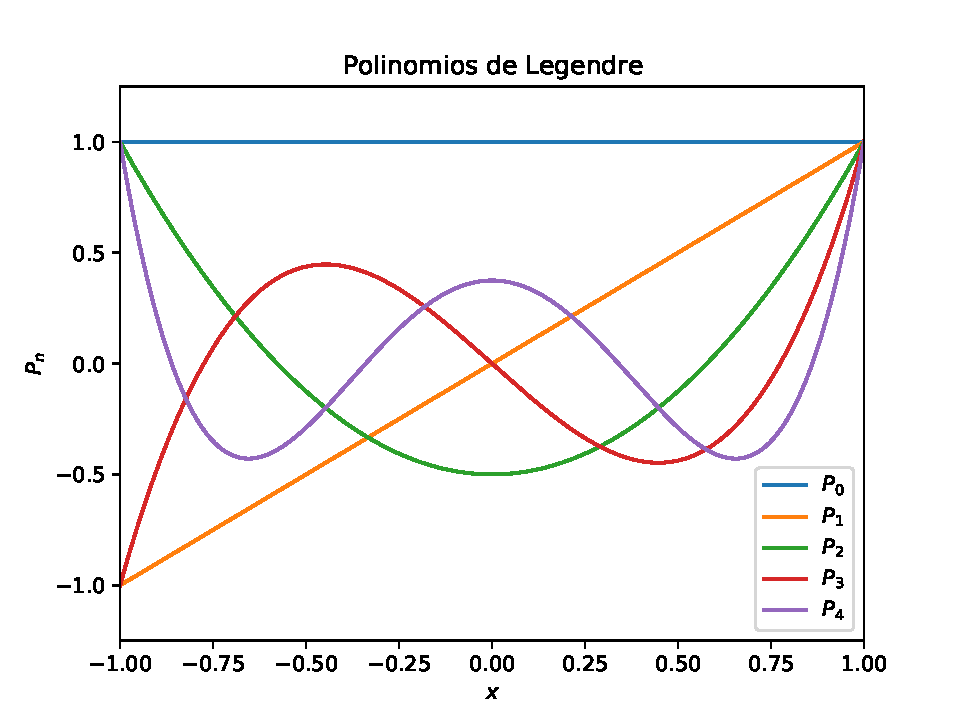
\includegraphics[scale=0.65]{./img/polinomiosLegendre.pdf}
	\caption{\href{https://github.com/DSarceno/Other/blob/main/Stuff/pLegrende.py}{Gráfico} de los primeros $5$ polinomios de Legendre.}
\end{figure}




\begin{mdframed}[style=warning]
	{\Large \textbf{Series de Legendre:}} \\
	Dada la ortogonalidad de los polinomios de Legendre, es narutal verlos como una base. Con esta idea y la de Fourier, se tiene que para una función definida en el rango $(-1,1)$
		$$ f(x) = \sum _{n = 0} ^\infty a_n P_n (x), $$
	con los coeficientes de fourier, dados por
		$$ a_n = \frac{2n + 1}{2} \int _{-1} ^1 f(x) P_n (x) \dd{x}. $$
	Un pequeño ejemplo es la solución a la ecuación de Laplace en coordenadas esféricas.
\begin{equation}
	\psi (r,\theta ,\varphi) = \sum _{l,m} \qty(A_{lm} r^l + B_{lm} r^{-l-1}) P_l ^m (\cos{\theta}) \qty(A_{lm} ' \sin{m\varphi} + B_{lm} ' \cos{m\varphi}) , \label{sollaplace}
\end{equation}
	donde $P_l ^m (x)$ son los \textbf{polinomios asociados de Legendre} y tienen la siguiente forma
		$$ P_l ^m (x) = (-1)^m \qty(1 - x^2)^{m/2} \dv[m]{x} \qty(P_l (l)). $$
\end{mdframed}




La parte de fórmulas de recurrencia lo vieron en clase y lo repasarán bastante con la hoja de trabajo (\href{https://github.com/DSarceno/Auxiliatura/tree/main/Metodos\%20Matematicos/Hojas}{\textit{ejercicios23-6}}), así que me tomaré la libertad de dar unos pequeños ejemplos de aplicaciones de los polinomios de Legendre.



\subsection*{Solución a la Ecuación de Laplace}


\begin{mdframed}[style=warning]
	{\Large \textbf{Campo Gravitacional de la Tierra:}} \\
	Dado que la fuerza gravitacional es de cuadrado inversa, su potencial en regiones sin masa satisface la ecuación de Laplace, por ende, el potencial puede ser escrito en una forma simplificada de \eqref{sollaplace}
		$$ U(r,\theta) = \frac{GM}{R} \qty[\frac{R}{r} - \sum _{l = 2} ^\infty a_l \qty(\frac{R}{r})^{l + 1} P_l (\cos{\theta})]. $$
	En donde el primer término de esta expansión describe si la tierra fuera esférica, el resto de términos describen las distorciones. Se conocen hasta $a_{20}$.
\end{mdframed}



\begin{mdframed}[style=warning]
	{\Large \textbf{Esfera en un Campo Uniforme:}} \\
	El ejemplo clásico y el primero que se estudia es el de una esfera conductora se encuentra en un campo eléctrico de magnitud $E_o$. El nuevo problema es encontrar el nuevo campo perturbado debido a la esfera. Utilizando las condiciones de frontera correctas y realizando el desarrollo mostrado en referencia ($1$), p728. Se tiene que la solución es
		$$ \psi (r, \theta) = -E_o z \qty(1 - \frac{r_o ^3}{r^3}). $$
\end{mdframed}










\pagebreak


\section*{Problemas}



\begin{ejercicio}
	En la guía $1$ se dejó el problema de demostrar que para los polinomios de Legendre se cumple lo siguiente:
		$$ \int _{-1} ^1 P_n ^2 (x) \dd{x} = \frac{2}{2n + 1}, $$
	para lo cual se dio como \textit{hint} una de las fórmulas de recurrencia. Ahora, demuestre lo mismo, sin utilizar las fórmulas de recurrencia.
\end{ejercicio}


\begin{ejercicio}
	Expanda $x^8$ como una serie de Legendre.
\end{ejercicio}



\begin{ejercicio}
	Obtenga, como una expansión de Legendre, el potencial electroestático de un anillo circular del ejemplo 15.2.3. (\textit{Arfken}, p733.), para puntos $(r,\theta)$ con $r < a$.
\end{ejercicio}














%%%%